\documentclass[12pt, a4paper]{article}
% including images
\usepackage{graphicx}
\usepackage[margin=1in]{geometry}
\graphicspath{ {./figs/} }

% For links
%\usepackage{hyperref}
% For indent after new heading 
\usepackage{indentfirst}

% citations
\usepackage[backend=biber,style=ieee]{biblatex}
\addbibresource{report.bib}
% Chinese typesetting
\usepackage{xeCJK}
\setCJKmainfont{WenQuanYi Micro Hei Mono}
\usepackage{setspace}

\begin{document}
\newcommand{\largeTitle}[1]{\fontsize{40}{50} #1}

%---------- TITLE PAGE ---------- 
% TODO: Fix the fonts to make it more professional
\begin{titlepage}
		\begin{center}
			\vskip 1.0cm
			\largeTitle \textbf{國立交通大學} \\[0.25cm]
			\largeTitle \textbf{資訊工程學系} \\[0.25cm]

			\LARGE{飛行器應用之54智慧2D影像拼接技術} \\[0.5cm]

			\LARGE{Intelligent Image Processing for Aerial 2-D Image Stitching}
		\end{center}

		\vspace{\fill}
		% bottom half of title page
		% TODO: This looks quite weird
		\begin{tabular}{c l}
				{\makebox[8em][s]{\LARGE 大學生:}} & \LARGE 彭思安(0616110) \\[0.5cm]
			{\makebox[8em][s]{\LARGE 指導教授:}} & \LARGE 楊啟瑞 \\[0.5cm]
		\end{tabular}

		\vspace{3cm}
		% TITLE PAGE FOOTER
		\begin{center}
			{\LARGE 中華民國 109 年 12 月 30日}
		\end{center}
\end{titlepage}

% ---------- ABSTRACT ----------
\section{Abstract}
\label{sec:Abstract}
Intelligent Image Processing is one of the subtask of 5G-DIVE Autonomous Drone Scout (ADS) verticals. It 
aims  to  intelligently  compute  drone  video  stream  in  the  edge  to  detect  persons  in  need  of  help,  and  to 
provide stitched image of a disaster impacted area. 5G-DIVE project is a collaborative project between the 
EU  and  Taiwan  to  prove  the  technical  merits  and  business  value  preposition  of  5G  technologies  in  ADS 
vertical pilot. In this research project, we worked on an improved Aerial 2D-ST solution that leverages the 
5G-DIVE platform specifically the IESS to improve 2D-ST. In particular, AI techniques is used as a solution to 
improve on the existing 2D-ST solution to produce high-quality stitched image but without sacrificing for 
computation time.

\section{Introduction}
\label{sec:Introduction}
The 5G-DIVE project between Taiwan and the European Union aims to show the viability of 
5G and edge computing. The emphasis in NCTU involves using drones to scan disaster areas
for Persons in Need of Help(PiH). Once a PiH is located by a drone, another drone will 
start taking images from that area and sending them to a server for image stitching. 
The contribution this project aims to make is to tailor the pipeline for this specific
scenario, hopefully reducing the latency enough to perform image stitching in real-time.
Once the stitching is performed, some more information can be gained frome the area 
surrounding the PiH,  such as other PiH or a potential hazard. First, we provide a
preliminary introduction to the idea of image stitching.

A panorama in visual art depicts a continuous scene or landscape~\cite{Panorama}. 
The concept of panoramas in photoraphy has existed for centuries. 
In the middle of the 19$^{th}$ century, landscapes were created by placing daguerrotypes side by side
side by side~\cite{OhioStitching}. Panorama images have been popularized in the last
years due to their widespread inclusion in smartphones and digital cameras; for example,
the iPhone5 introduced panoramic images in 2012~\cite{iPhoneStitch}. As processing
power has grown, new and increasingly smart solutions have allowed better quality
images to be stitched for pleasing results.

In digital photography, a panoramic image refers to a large composite image made of 
smaller images with overlapping areas. 
Computer software will look for the optimal way to combine the overlapping areas of the 
images such that the output panorama exhibits little or no visual artifacts. 
Image stitching has multiple uses other than recreative or artistic, producing
a map of an area from overhead drone image~\cite{OpenDroneMapTheMissingGuide}, or 
for medical imaging applications.


\begin{figure}[b]
		\label{fig:PanoExample}
		\centering
		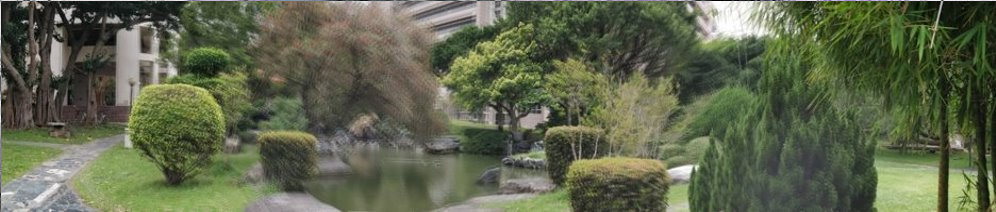
\includegraphics[scale=0.4]{pano.png}
		\caption{Example of stitched image consisting of six individual images. Some visual 
		artifacts such as blurring might remain in the final panorama.}
\end{figure}

\section{Problem Description}
\label{sec:ProblemDescription}
The problem of focus here involves designing and implementing an image stitching 
pipeline that is robust yet has low latency. The input will be a series of images
taken by a drone, and the output will be a single high-resolution panorama image.

An envisioned usage scenario would involve drones capturing video footage 
over an area impacted by some disaster. This footage is then to be transmitted 
to a server for stitching. Using the stitched images, a clearer representation of the 
impacted area should be visible, in case detecting persons in need of help or
producing a clearer picture of the area was necessary. 

The problem addressed in this paper involves taking a stream or set of images
of a specific area and outputs a single stitched image. The image is a composite
of the input images and their overlapping components. This pipeline should be 
robust and have as little latency as possible, since there will be a consistent
stream of images and the results should be viewed as soon as available. The current
objective is to have image stitching performed in a few seconds, or as close to 
real-time as possible.

\section{Existing Literature}
\label{sec:Literature}

The original paper on image stitching~\cite{brown2007automatic} introduces a 
pipeline with several steps: feature matching, image matching, bundle adjustment,
panorama straightening and blending. Many individual projects implement this 
pipeline and even some professional projects. OpenCV's image stitching module
utilizes this pipeline to stitch multiple images together.

Next is a brief description of the pipeline according to the original paper:
\begin{enumerate}
		\item \textbf{Feature Matching}: In this stage we find the regions of 
				interest in each image of the sequence. A region of interest,
				commonly called a feature, could represent an area of the image
				with large variations in pixel intensities. Once a feature is 
				found, relevant information about it is stored in a k-d tree.
				This k-d tree will store the points by their location in the 
				image, so lookups of physically nearby features can be done 
				in $O(\log(n))$ time~\cite{IntroToAlgorithms}.

		\item \textbf{Image Matching}: In this stage we find connected sets 
				of images which will be stitched together. To find appropriate
				pairs of images, the RANSAC algorithm is used. The algorithm
				will look at the probability that a certain match was generated
				by a correct image match.

		\item \textbf{Bundle Adjustment}: In the previous step, matching pairs
				of images had been calculated based on inlier features. In this 
				step, the bundle adjuster structure will adjust the camera parameters
				of each image added. This avoids cumulative errors resulting from the 
				homography estimation. When each subsequent image is added to the bundle,
				for each feature the error is calculated from that feature in the other 
				images. 
		\item \textbf{Panorama Straightening}: At this point, the image's parameters
				have been adjusted relative to each other;however in this step the 
				the global camera is taken into account. Since the sequence of pictures
				are probably not taken along a perfectly even plane, the null vector of the
				covariance camera matrix is used to ensure the images are all taken 
				in a single plane.
 
		\item \textbf{Blending}: Given a panorama picture, the last step involves softening
				the image edges. This is done by assigning a weight function to the overlapping
				regions, which depends on their position from the edge of the image. Thus there
				is a more gradual change in the pixel values from one image to the next.

\end{enumerate}

\begin{figure}
	\label{fig:PipelineOriginal}
	\centering
	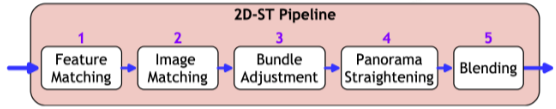
\includegraphics[scale=0.6]{pipeline_orig.png}
	\caption{2-D stitching pipeline based on original paper. The input consists of a set of images and the 
		output consists of a single, high-resolution image.}
\end{figure}

Since its publication this pipeline has been implemented in many open source alternatives, such
as OpenCV and many smaller projects. 

However, recently there have been newer methods that focus on improving certain parts of the pipeline. 
For example, the SuperGlue pretrained network~\cite{Sarlin_2020_CVPR} utilizes a neural network
to perform feature matching and image matching. 

\section{Resolution Method}
\label{sec:ResolutionMethod}
The current project took the pipeline in Section~\ref{sec:Literature} as a starting point. After
understanding the pipeline, its inputs and outputs at each step, and some possible ways of 
implementing it in code, it was clear that some improvements could be made. For our application,
the main focus was balancing the visual results with the latency. One of the first steps in the
procedure was timing each step in the pipeline to identify possible areas of improvement.

\begin{figure}
	%\centering
	\label{fig:PipelineTiming_orig}
	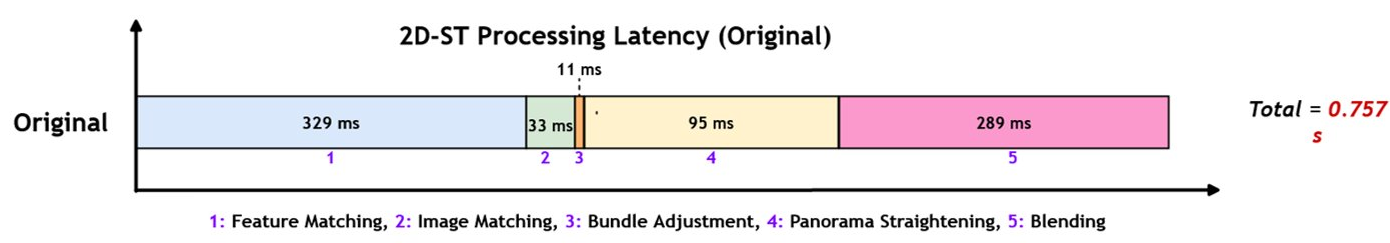
\includegraphics[scale=0.3]{pipelineTiming_orig.png}
	\caption{Timing diagram of first image stitching pipeline.}
\end{figure}

The program used to time the pipeline utilized OpenCV, since it offers variety of the 
funcitons and algorithms we need to implement the pipeline step by step. Initially, two
images were tested to determine the specific place where our program spent the longest 
amount of time. From Figure~\ref{fig:PipelineTiming_orig}, it was clear the 
feature matching and blending.

This finding prompted a search for methods to improve on the latency of the pipeline for our 
specific use case. Among them was SuperGlue pretrained network, which uses a neural network
to perform image matching and feature matching. The reason this project was chosen as a 
substitute for our original OpenCV implementation was due to its drastic improvement 
in terms of latency. In our original implementation, all the image processing ocurred at the 
image's native resolution and in full color. SuperGlue downsized the images to 640x480 resolution
down from the iamge's native 1920x1080 resolution. Besides the downsampling, the images
were also turned to greyscale for quicker processing of image data. 

With only some slight changes to the source code, this project was integrated 
into the rest of the pipeline. 
Since the rest of our project was based around the OpenCV implementation, the programs output 
had to be compatible with the  rest of the pipeline. Fortunately, this was not a problem
since the model's output was of type \texttt{numpy.ndarray} which could easily be turned to
\texttt{cv2.KeyPoint()} as was needed in the second step of the pipeline.

As a next step, an alternative blending method could also be researched. In the years since,
there likely is a more efficient way of performing the blending process.

\section{System Design and Implementation}
\label{sec:DesignAndImplementation}

A major focus of the process involved testing the latency of each stage in the pipeline.
The testing was performed only on two images, since the focus of the latency testing
required us to identify the most time-consuming steps in our pipeline. The program
was restructured in order to perform this. The original  pipeline program was written
such that it was all in a single file. For latency testing, the pipeline was split into
each stage. This way we could easily measure the latency on one single task.

Figure~\ref{fig:tree} shows the directory structure used to test the latency. Each subdirectory
contains an \texttt{input/} and \texttt{output/} subdirectory, along with a \texttt{main.py}
script. The code in each stage was refactored such that each \texttt{main.py} script would
take the required inputs from the previous stages and once finished, write its output to
the \texttt{output/} directory. In this manner we could straightforwardly use a Python timer, 
alongside the \texttt{time} command to carry out the latency testing for each stage.


\begin{figure}
	\label{fig:tree}
		\centering
		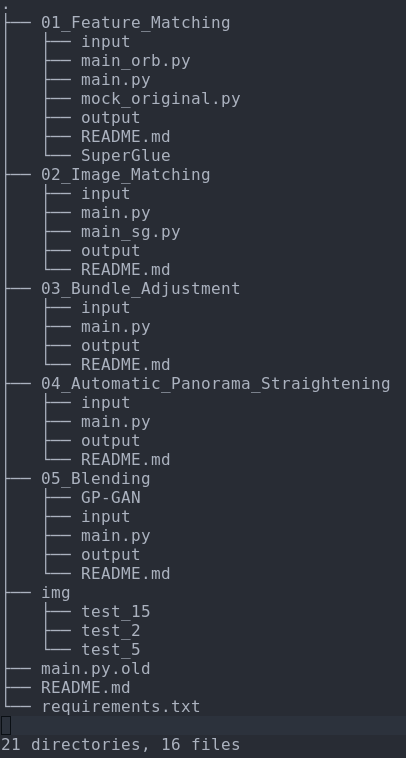
\includegraphics[scale=0.4]{dir.png}
		\caption{Main directory structure. There is a directory for each stage, with 
		an \texttt{input} and \texttt{output} subdirectories where associated files are 
		read from and stored to.}
\end{figure}

When the final pipeline is to be implemented, the structure will most likely be 
a single script that executes all the steps of the pipeline.
\section{Result Analysis}
\label{sec:Results}

The timing performance was performed by running the same pair or set of images using both
methods. First, we just were concerned only with the first step of the pipeline, the
feature matching stage. The \texttt{input/} folder contains merely the images to be stitched.
The normal \texttt{main.py} script will utilize the original pipeline design with SIFT to 
perform feature matching. The \texttt{SuperGlue/} directory contains the software project for
the alternative neural network method.

In order to use the results from the step, the output files were written to the \texttt{output/}
directory, where they were then used by the folder corresponding to the next step in the 
pipeline. There still remains some work to be done in integrating the result of the network
with the rest of the pipeline, specifically referring to the format of the outputs from the 
feature matching stage. Despite this, early results indicate the possibility of a substantial
reduction in the stitching latency.

\begin{figure}
	\centering
	\label{fig:TimingComparison_comp}
	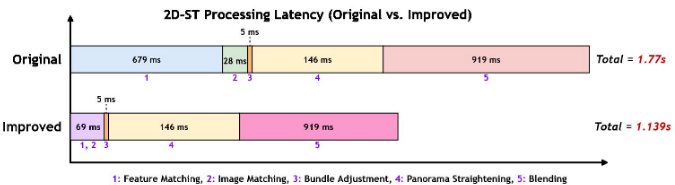
\includegraphics[scale=0.6]{timing_comp.png}
	\caption{Timing results for the original SIFT-based feature matching method and the 
		SuperGlue pretrained network.}
\end{figure}

Based on Figure~\ref{fig:TimingComparison_comp}, implementing the neural network method for
feature matching resulted in around an $80\%$ reduction in latency. As mentioned, this 
promising first result could lead to further reduction in latency for future stages in the
stitching pipeline, particularly the blending stage, which after feature matching is the 
longest stage.

\section{Conclusions and Contributions}
\label{sec:Conclusion}
In conclusion, the image stitching pipeline can be optimized for our use case. By using some
more recent methods involving AI, the latency of previously intensive steps can be reduced 
significantly. In the future, we hope this method can be used in near real-time in the 5G-DIVE
project. While there are still many technical considerations to be resolved before this 
project's implementation, there has already been some promising progress so far.

The 5G-DIVE project involves controlling multiple drones and their feed to perform person
detection, and subsequently image stitching. The image stitching component constitutes a small
part of the overall project. 

To this end, this project would not have been possible without the edifying criticism and 
guidance from my advising professor, 楊啟瑞. Although she rarely takes undergraduate 
students, she made an exception for me and this opportunity would not have been possible 
otherwise. Also, a heartfelt thanks is in order to the students in her lab, Timothy William and
Muhammad Febrian Ardiansyah, who patiently helped me write bi-weekly progress reports and 
assisted with the requirements for this course.

\section{Future Steps}
\label{sec:FutureSteps}
Since the 5G-DIVE project is still ongoing, there are some considerations that need to be 
addressed before this project can officially be considered as finished. For example, the input
images to the stitching module will come from a drone that is continually shooting images. 
If we stitch images that were taken almost at the same time the difference might not be 
noticable, it would be a misuse of processing time. Thus we need to find the optimal rate 
at which to stitch images, e.g. every third image in a stream of images. 

Another remaining consideration involves investigating progressive stitching. By this, we mean
that instead of stitching the images completely from zero every time, we could hold a panorama
image and cumulatively stitch that panorama image with incoming images. This way we would only
be required to stitch few images per iteration. The possible drawback in this scenario could
be the distortion or visual artifacts remaining after every iteration. These might be compounded
if we used the same panorama image repeatedly in multiple iterations.

In terms of challenges, the largest one involved stitching regions of a building side without
much changes. Many of the datasets that were tested varied too little between each image. 
Also, since the building sides contained many of the same features in different regions of the 
image, the pipeline struggled to determine where each region was supposed to be stitched. As
a result, some regions of interest were left out of the image completely.
\vspace{\fill}

\erintbibliography
\end{document}

